\chapter{Sample Problem}
\label{chapter:sample-problem}

In order to validate the different modules of \texttt{hIPPYfire}, one of \texttt{hIPPYlib}'s Bayesian inversion test cases, namely \texttt{3-SubsurfaceBayesian} \cite{Villa_hIPPYlib_An_Extensible_2020}, was recreated. This test case utilized all of \texttt{hIPPYfire}'s models that have been currently developed. Additional test cases shall be added for future functionality. The test case is briefly discussed below; a detailed description of the test case can be found in \texttt{hIPPYlib}'s repository \cite{Villa_hIPPYlib_An_Extensible_2020}.

This test case solves the forward problem and computes the MAP point, as described in Section \ref{chapter: inverse-problems}. The forward problem of this test case is governed by an elliptic PDE. The objective is to compute the parameter fields with a certain probability that these gave rise to the observed data. Please note that the following test case admits discretized expressions of the parameter space, i.e., they are finite-dimensional.

A Gaussian prior is assumed with a mean of $\textbf{m}_{prior}$. Its covariance, \textbf{$\Gamma_{prior}$}, is obtained by discretizing the inverse of the differential operator $\mathcal{A}^{-2} = (-\gamma\Delta + \delta\textbf{I})^{-2}$, where $\gamma, \delta > 0 $. The prior is chosen such that the well-posedness of this problem is ensured.

The likelihood is calculated as shown below:
\begin{equation}
    \textbf{d}_{obs} = \textbf{f(m)} + \textbf{e}
\end{equation}
$\textbf{e}$ represents the noise, which is computed by the \texttt{randomGen()} method in the \texttt{rand} module.
\begin{equation}
    \pi_{like}(\textbf{d}_{obs} | \textbf{m}) = exp(-\frac{1}{2}(\textbf{f(m)} -\textbf{d}_{obs})^T\Gamma^{-1}_{noise}(\textbf{f(m)} -\textbf{d}_{obs}))
\end{equation}

The above equation presents a discretized version of the likelihood function. The mean of the posterior distribution, also referred to as \textbf{${m_{MAP}} $}, is the parameter vector that maximizes the posterior. Its discretized computation is listed below:
\begin{equation}
    \textbf{m}_{MAP} := \underset{m}{arg min}\mathcal{J}(\textbf{m}) := (\frac{1}{2} || \textbf{f(m)} - d_{obs} ||^2_{\Gamma_{noise}^{-1}} + \frac{1}{2}|| \textbf{m} - \textbf{m}_{prior} || ^2_{\Gamma_{noise}^{-1}}
\end{equation}

Problem flow has been defined until the computation of the MAP point in \texttt{hIPPYfire}. A few code snippets have been included below

\begin{itemize}
    \item \textbf{Mesh and FEM setup}: A two-dimensional unit square mesh is created with a P2 finite element space for \texttt{state} and \texttt{adjoint} variables and P1 for \texttt{parameter}.
    \begin{lstlisting}[language=python]
        ndim = 2
        nx = 64
        ny = 64
        mesh = fd.UnitSquareMesh(nx, ny)
        Vh2 = fd.FunctionSpace(mesh, 'Lagrange', 2)
        Vh1 = fd.FunctionSpace(mesh, 'Lagrange', 1)
        Vh = [Vh2, Vh1, Vh2]
    \end{lstlisting}
    \item \textbf{Forward Problem}: As mentioned in Section \ref{chapter: software}, the \texttt{PDEVariationalProblem} class sets up the forward problem component of the \textit{p2o} map. In addition to the finite element components defined above, it requires an expression of the weak form of the PDE (given by \texttt{pde\_varf}) and boundary conditions for the forward (\texttt{bc}) and incremental and adjoint problems (\texttt{bc0}).
    The \texttt{PDEVariationalProblem} class solves the forward/adjoint and incremental problems and computes the relevant partial derivatives with respect to the state, parameter, and adjoint variables.
    \begin{lstlisting}[language=python]
        u_bdr = fd.SpatialCoordinate(mesh)[1]
        u_bdr0 = fd.Constant(0.0)

        bc = fd.DirichletBC(Vh[STATE], u_bdr, [3, 4]) # [3, 4] indicates that bc is applied to y == 0 amd y ==1
        bc0 = fd.DirichletBC(Vh[STATE], u_bdr0, [3, 4])

        f = fd.Constant(1.0)

        def pde_varf(u, m, p):
            return ufl.exp(m) * ufl.inner(ufl.grad(u), ufl.grad(p)) * ufl.dx - f * p * ufl.dx

        pde = PDEVariationalProblem(Vh, pde_varf, bc, bc0, is_fwd_linear=True)
    \end{lstlisting}
    The \texttt{is\_fwd\_linear=True} flag allows the user to set a non-linear forward map as well.
    \item \textbf{Prior setup}: The class \texttt{BiLaplacianPrior} creates a Gaussian prior with zero average, Additional information regarding the covariance can be found in Villa et al. \cite{Villa_hIPPYlib_An_Extensible_2020}.
    \begin{lstlisting}[language=python]
        pr = BiLaplacianPrior(Vh[PARAMETER], gamma, delta, robin_bc=True)
        x = fd.SpatialCoordinate(mesh)
        mtrue = fd.interpolate(fd.sin(x[0])*fd.cos(x[1]), Vh[PARAMETER]).vector()
        m0 = fd.interpolate(fd.sin(x[0]), Vh[PARAMETER]).vector()
        objs = [fd.Function(Vh[PARAMETER], mtrue), fd.Function(Vh[PARAMETER], pr.mean)]
    \end{lstlisting}
    The true parameter, \texttt{mtrue} is initialized to be a known analytic function to validate the accuracy of the parameters cmoputed by \texttt{hIPPYfire}. Plots of the vectors \texttt{mtrue} and \texttt{pr.mean} are generated and shown below. For the purpose of validation through this test case, \texttt{mtrue} is a known function and not randomly generated, as in \texttt{hIPPYlib} \cite{Villa_hIPPYlib_An_Extensible_2020}
        \begin{figure}[th]
        \centering
        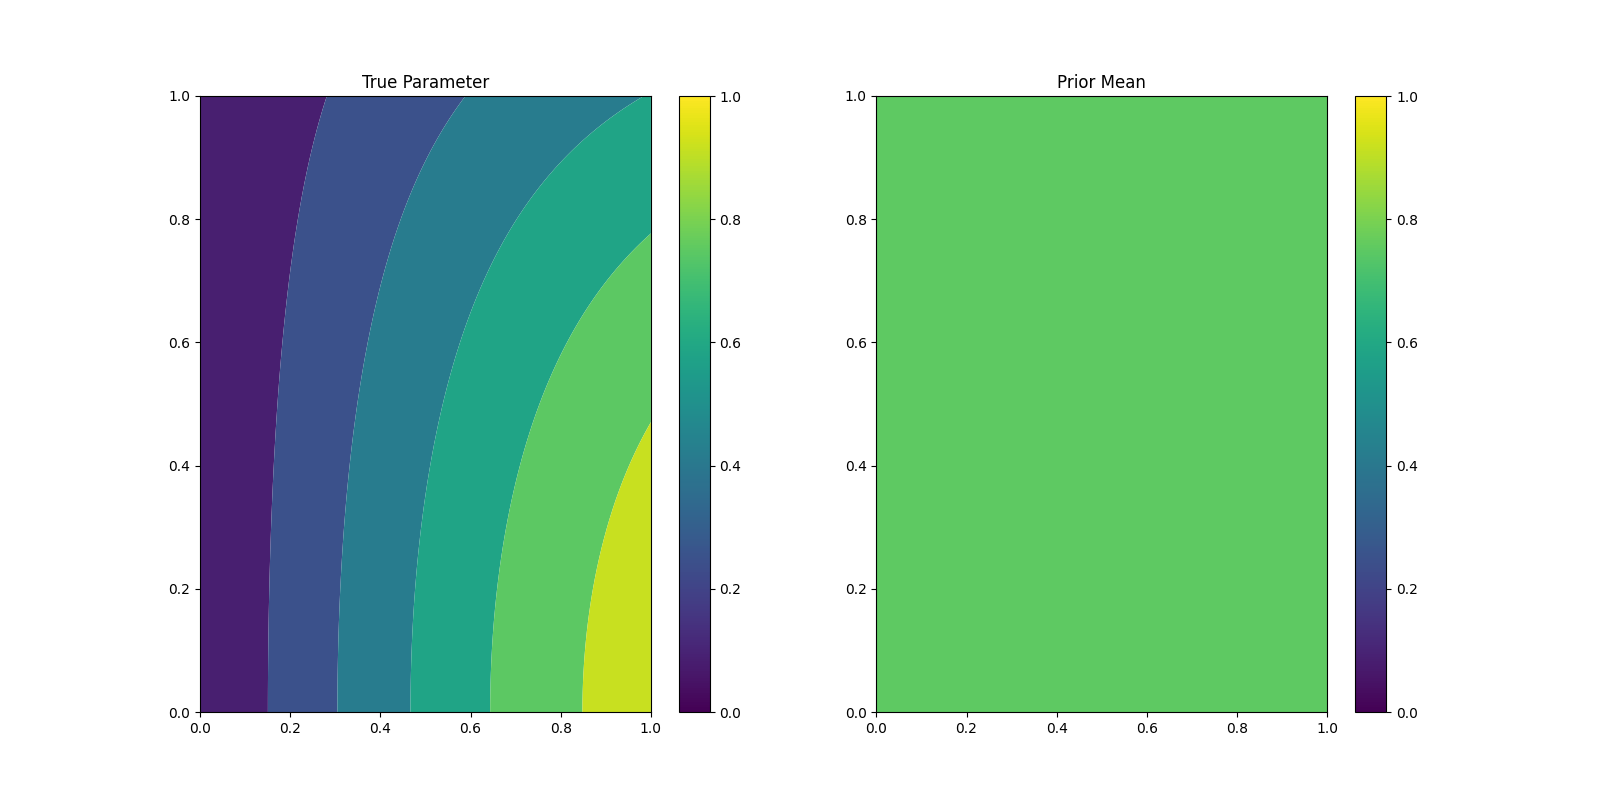
\includegraphics[width=1.0\textwidth]{figures/parameter.png}
        \caption{Variation of the true parameter and mean.}
        \label{figure:parameter}
        \end{figure}
    \item \textbf{Misfit}: \texttt{hIPPYfire} currently provides support for \texttt{ContinuousStateObservation}, which sets up the observation parameter $\mathcal{B}$. The observables which shall provide our input data are first generated by solving the forward problem by using the true parameter $\textbf{m}_{true}$
    \begin{lstlisting}[language=python]
        misfit = ContinuousStateObservation(Vh[STATE], ufl.dx, bcs=bc0)
        misfit.noise_variance = 1e-4
        utrue = pde.generate_state()
        x = [utrue, mtrue.vector(), None]
        pde.solveFwd(x[STATE], x)
        misfit.d.axpy(1., utrue)
        misfit.d.axpy(float(np.sqrt(misfit.noise_variance)), randomGen(Vh[STATE]).vector())
    \end{lstlisting}
    \begin{figure}[th]
        \centering
        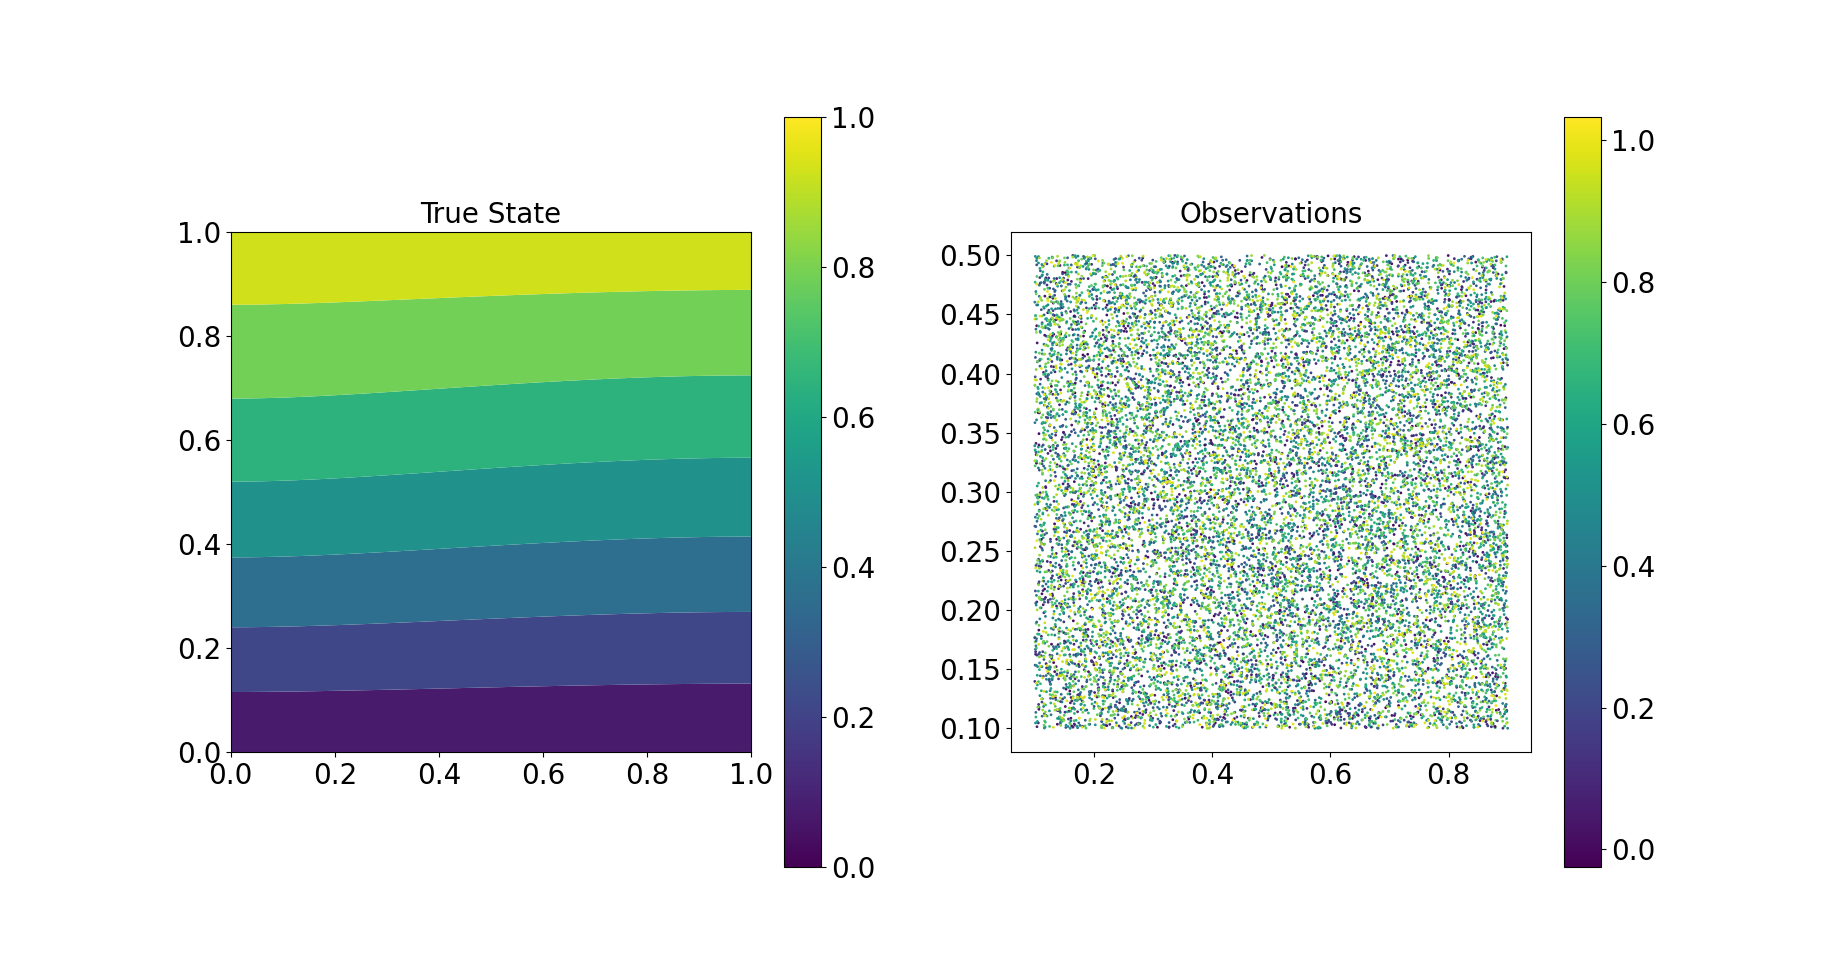
\includegraphics[width=1.0\textwidth]{figures/observations.png}
        \caption{Variation of the true state and the observations.}
        \label{figure:state}
    \end{figure}
    \item \textbf{Model}: The model, which is created by the \texttt{model} class, depends on three components---namely \texttt{PDEVariationalProblem}, \texttt{misfit}, and \texttt{prior}. The \texttt{PDEVariationalProblem} provides solutions for the forward and adjoint problems and incremental forward and adjoint problems. The \texttt{prior} applies the regularization operator to a vector, while the \texttt{misfit} computes the cost functional and partial derivatives with respect to the state and parameter variables.
    Forward finite differences are used to test the model through the \texttt{modelVerify} module.
    \begin{lstlisting}[language=python]
        model = Model(pde, pr, misfit)
        eps, err_grad, err_H = modelVerify(model, m0, misfit_only=False)
    \end{lstlisting}
    \begin{lstlisting}[language=bash]
        (yy, H xx) - (xx, H yy) =  0.0
    \end{lstlisting}
    \begin{figure}[th]
        \centering
        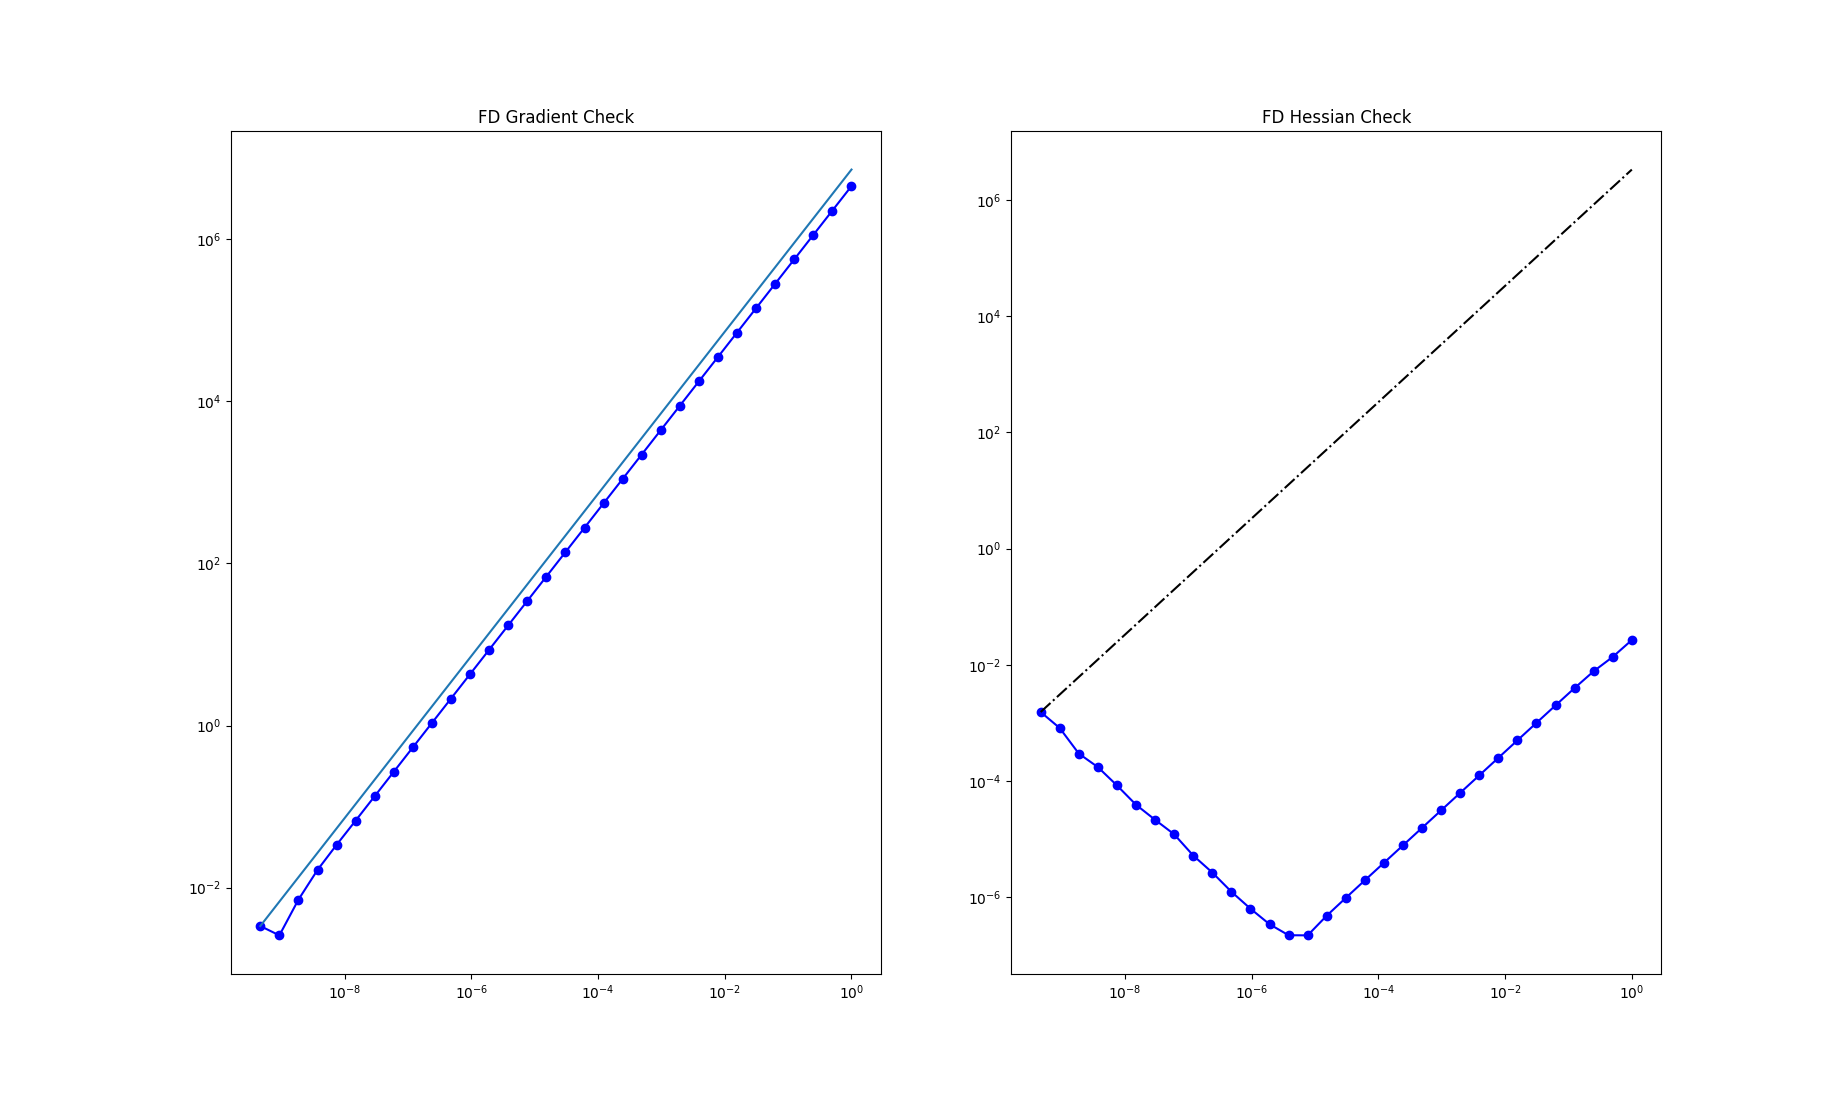
\includegraphics[width=1.0\textwidth]{figures/modelVerify.png}
        \caption{Gradient and Hessian Checks obtained from \texttt{modelVerify}}
        \label{figure:modelVerify}
    \end{figure}
    \item \textbf{MAP Point}: The Newton-CG method is used to compute the MAP point.
    \begin{lstlisting}[language=python]
        m = pr.mean.copy()
        solver = ReducedSpaceNewtonCG(model)
        solver.parameters["rel_tolerance"] = 1e-6
        solver.parameters["abs_tolerance"] = 1e-12
        solver.parameters["max_iter"]      = 25
        solver.parameters["GN_iter"] = 5
        solver.parameters["globalization"] = "LS"
        solver.parameters["LS"]["c_armijo"] = 1e-4
        x = solver.solve([None, m, None])
    \end{lstlisting}
    The following output was obtained:
    \begin{lstlisting}[language=bash]
        Relative/Absolute residual less than tol
Converged in  19  iterations with final norm  5.65259722013104e-08

It  cg_it cost            misfit          reg             (g,dm)          ||g||L2        alpha          tolcg         
1   1    9.452277e-01    8.990612e-01    4.616652e-02   -2.456844e+01   1.685316e+02   1.000000e+00   5.000000e-01
2   2    4.228824e-01    3.488744e-01    7.400803e-02   -1.043988e+00   1.715492e+01   1.000000e+00   3.190463e-01
3   5    4.027649e-01    3.196818e-01    8.308311e-02   -4.042007e-02   3.036538e+00   1.000000e+00   1.342297e-01
4   7    4.026241e-01    3.196381e-01    8.298594e-02   -3.009693e-04   2.404168e-01   1.000000e+00   3.776954e-02
5   7    4.026228e-01    3.196101e-01    8.301271e-02   -2.859017e-06   1.569884e-02   1.000000e+00   9.651461e-03
6   8    4.026228e-01    3.196134e-01    8.300935e-02   -4.118272e-08   8.007385e-04   1.000000e+00   2.179740e-03
5.941225051879883 Executiion time

Converged in  6  iterations.
Termination reason:  Norm of the gradient less than tolerance
Final gradient norm:  7.784347671669573e-06
Final cost:  0.40262278305284716
    \end{lstlisting}
    \begin{figure}[th]
        \centering
        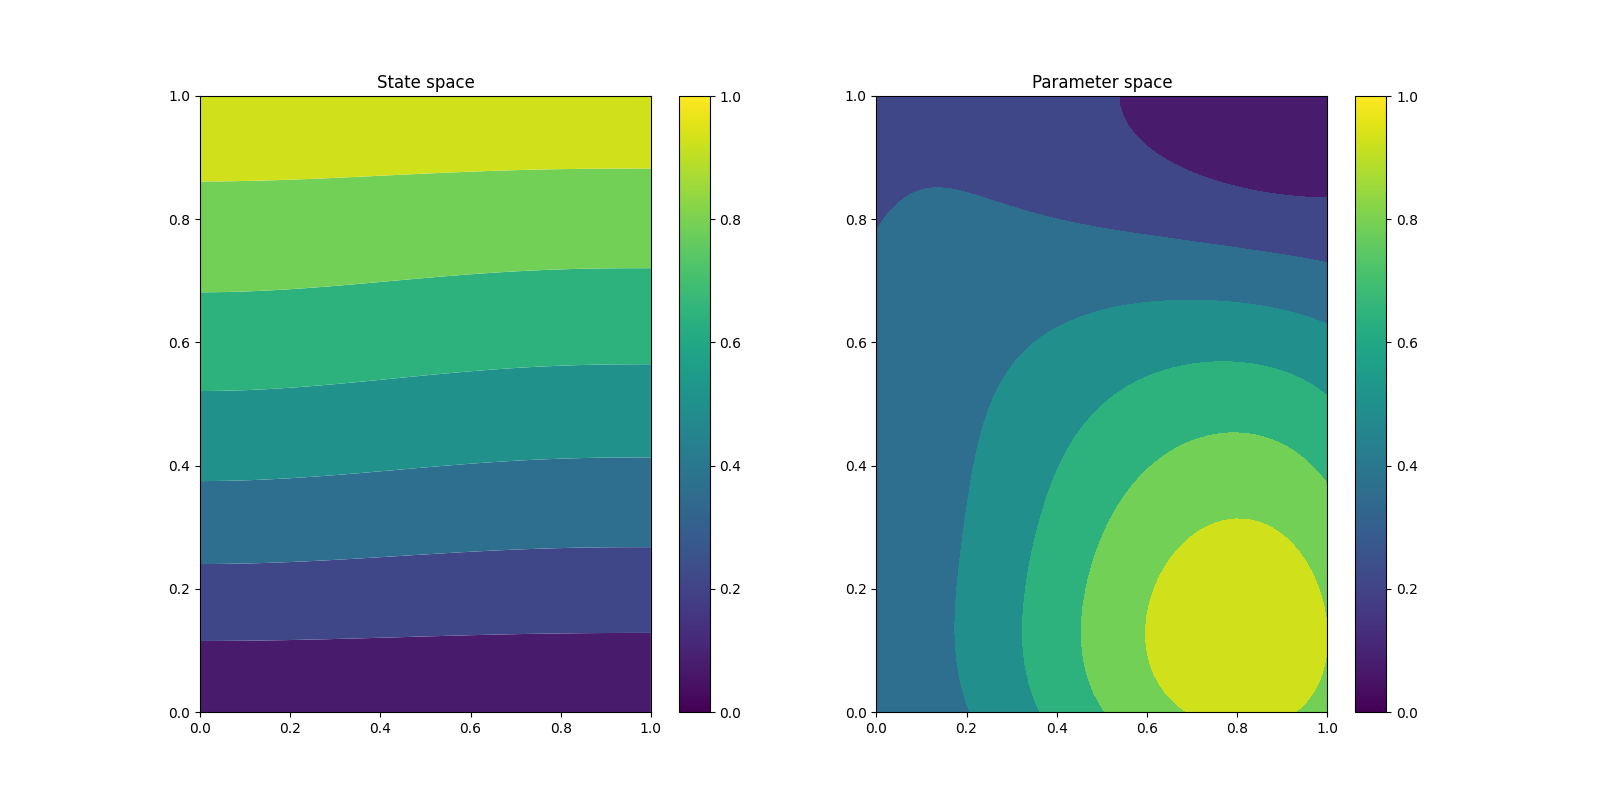
\includegraphics[width=1.0\textwidth]{figures/space.png}
        \caption{Contours of the state and parameter}
        \label{figure:space}
    \end{figure}
    A mesh independence study was conducted to establish that the convergence of the problem is observed for different sizes. The current sample assumes a uniform square mesh with 64 divisions. Experiments were conducted for mesh sizes of 128 and 256 divisions. Convergence was reported for 6--7 iterations for all mesh sizes. 
\end{itemize}